% !TeX root = ../main.tex
% Add the above to each chapter to make compiling the PDF easier in some editors.

\chapter{Methods}\label{chapter:introduction}
In the following the model used in this thesis as well as the applied training concepts are presented

\section{Model}
The model used during the experiments consists of a 1D CNN which is responsible to extract expressive features and a subsequent classifier predicting the health condition classes of the BSD. A more detailed. visualization of the architecture is shown in fig.\ref{fig:proposed_model}. The CNN consists of 3 convolutional layers. With increasing network depth the kernel size is decreased and padding size increased. This helps to extract more general and global features in shallow and more specific and local features in deeper layers. The exact parameters of the convolutional layers are described in table \ref{tab:parameter_conv} 

\begin{longtable}{||c c c c||} 
\hline
& Conv 1 & Conv 2 & Conv 3 \\
\hline
kernel size & 100 & 10 & 5 \\
\hline
padding size & 0 & 1 & 1 \\
\hline
stride & 1 & 1 & 1 \\
\hline
\caption {Parameter convolutional layer}
\label {tab:parameter_conv}
\end{longtable}

Several pooling layers are inlcuded to reduce after the convolutional layers. By reducing the complexity of the model 
problems of overfitting and exploding gradients are prevented. Applying batch normalization after convolutional layers fixes the means and variances of the layers inputs for each batch, which helps to make the training faster and more stable. After iteratively applying these three types of layers the output of the CNN is flattened and normalized to a 1D vector. This vector is used as an input for the subsequent classifier. The latent space dimension  of the classifier is reduced constantly. The two neurons in the output layer of the neural network represents the prediction probability for the two defined health condition classes.


\begin{figure}[H]
  \centering
  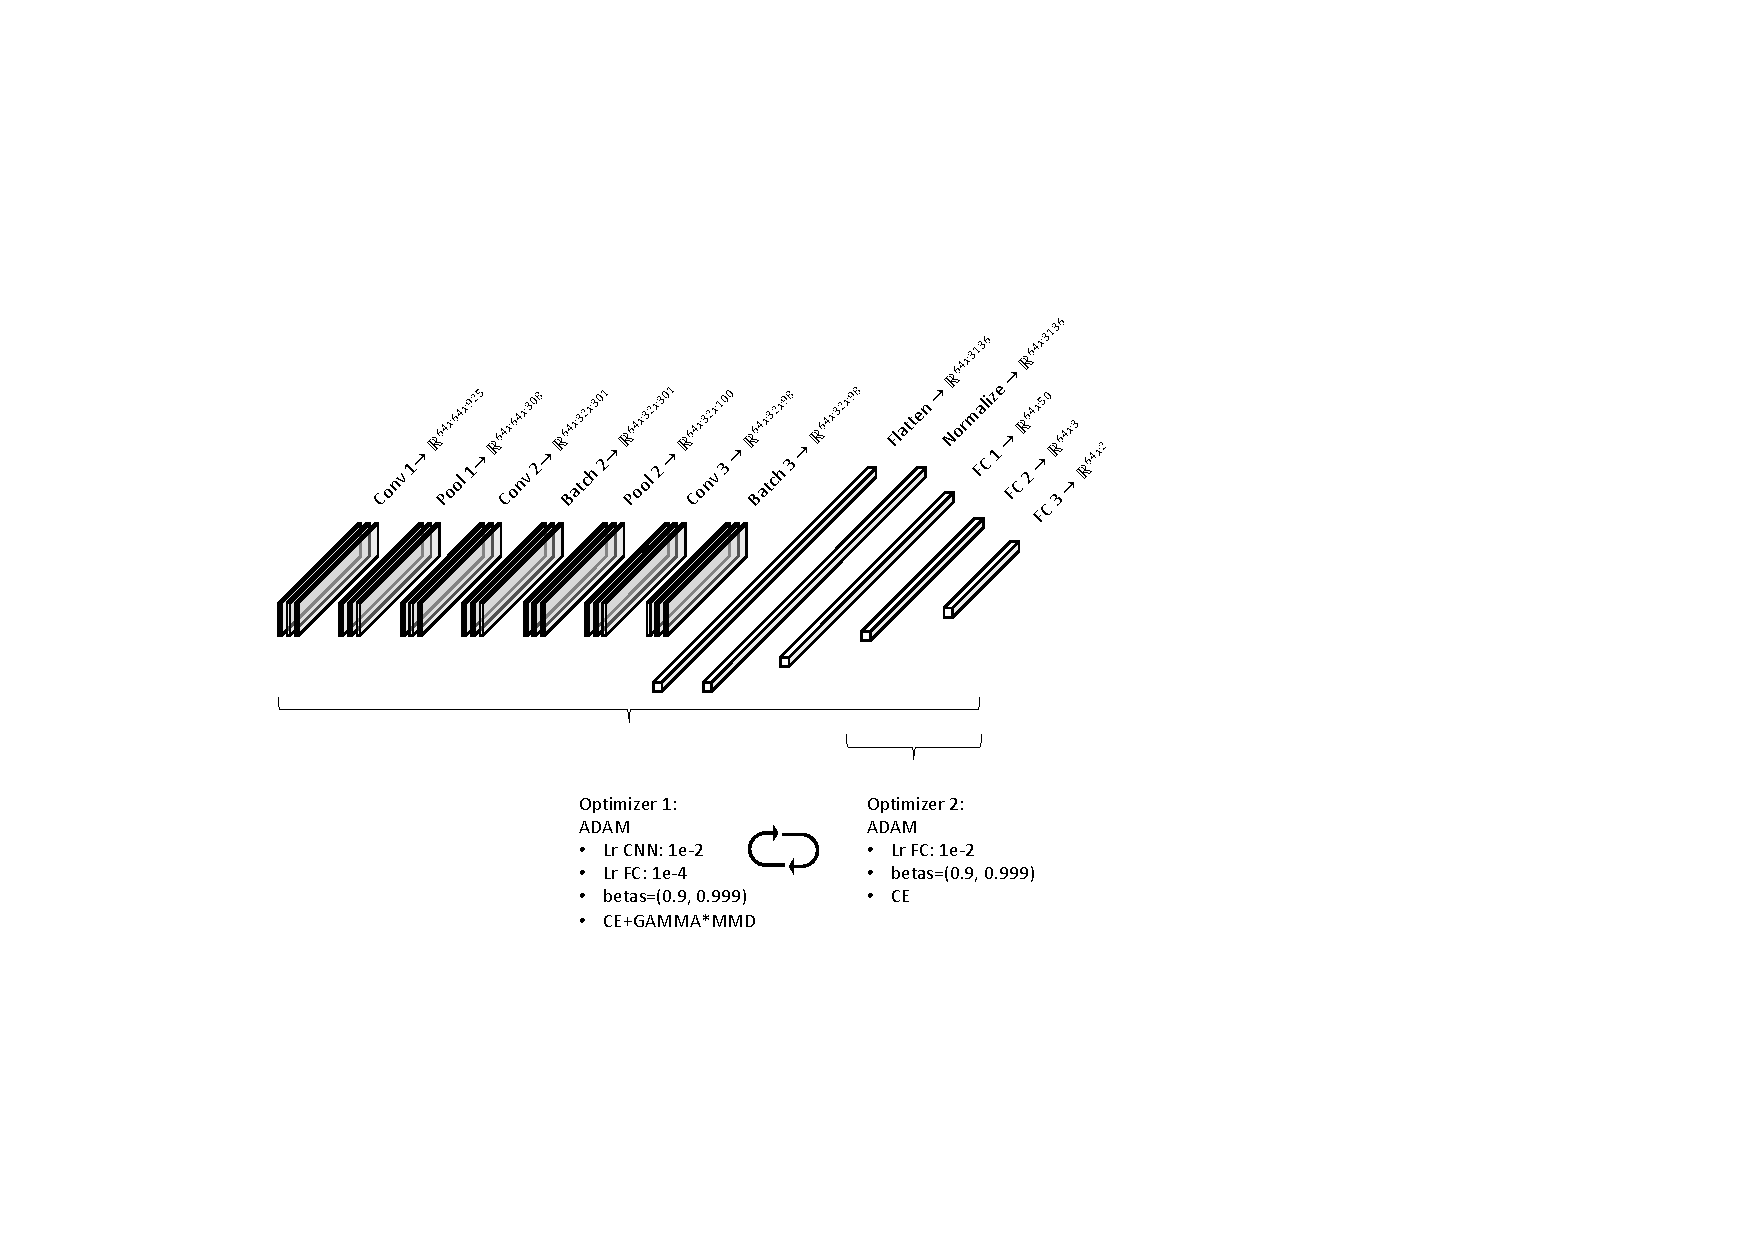
\includegraphics[width=1\textwidth]{proposed_model.pdf}
  \caption {Proposed model} \label{fig:proposed_model}
\end{figure}


\section{Proposed training with MMD and cross entropy loss} \label{sec:Proposed_training}

Firstly, the data used for the training is pre-processed. A data loader is used to prepare the data set. In a first step the data is separated in shorter sequences of length 1024. These windows, which can include several of the recorded 49 features, are fed as single samples to the model. The sequences are cleaned from Nan values and synchronized afterwards. The data set is randomly separated in a train, validation and test set with a split of 60\%/20\%/20\%. Also the application of wavelet transforms, which can generate more informative data for the model, were partially investigated in this step. The repetitive training of the model is visualized in fig. \ref{fig:Training_Process_MMD}. A combination of a source cross-entropy and MMD loss is is applied to optimize the proposed deep-learning based domain adaption model. The MMD loss estimates the domain discrepancy measured in several latent feature maps of. The MMD loss facilitates the extraction of more domain independent features within the model's layers. The cross entropy loss trains the model to increase the classification accuracy on the source domain. The domain discrepancy is measured as squared distance between between distribution kernel embeddings in the reproducing kernel Hilbert space (RKHS). For the performance of the MMD loss the kernel choice is of great importance. For this reason several RBF kernels with bandwidth parameters 1, 2, 4, 8, 16 were combined in order to profit from their individual strength. For applying the MMD loss two samples from each, source and target domain, are sampled randomly. For each such generated pair of samples is processed the MMD loss is calculated. The class of each sample is not considered during in the MMD loss. Therefore, the MMD loss minimizes the domain discrepancy based on the observed source and target domain sample pairs which partially belong to different but also to the same BSD health condition classes. The MMD is applied in several layers of the CNN and classifier. The source cross entropy loss is applied in the final layer. Fig. \ref{fig:MMD_Loss_and_CE_loss} symbolically shows how the MMD and the source cross-entropy loss is extracted from the different layers of the model.

\begin{figure}[H]
  \centering
  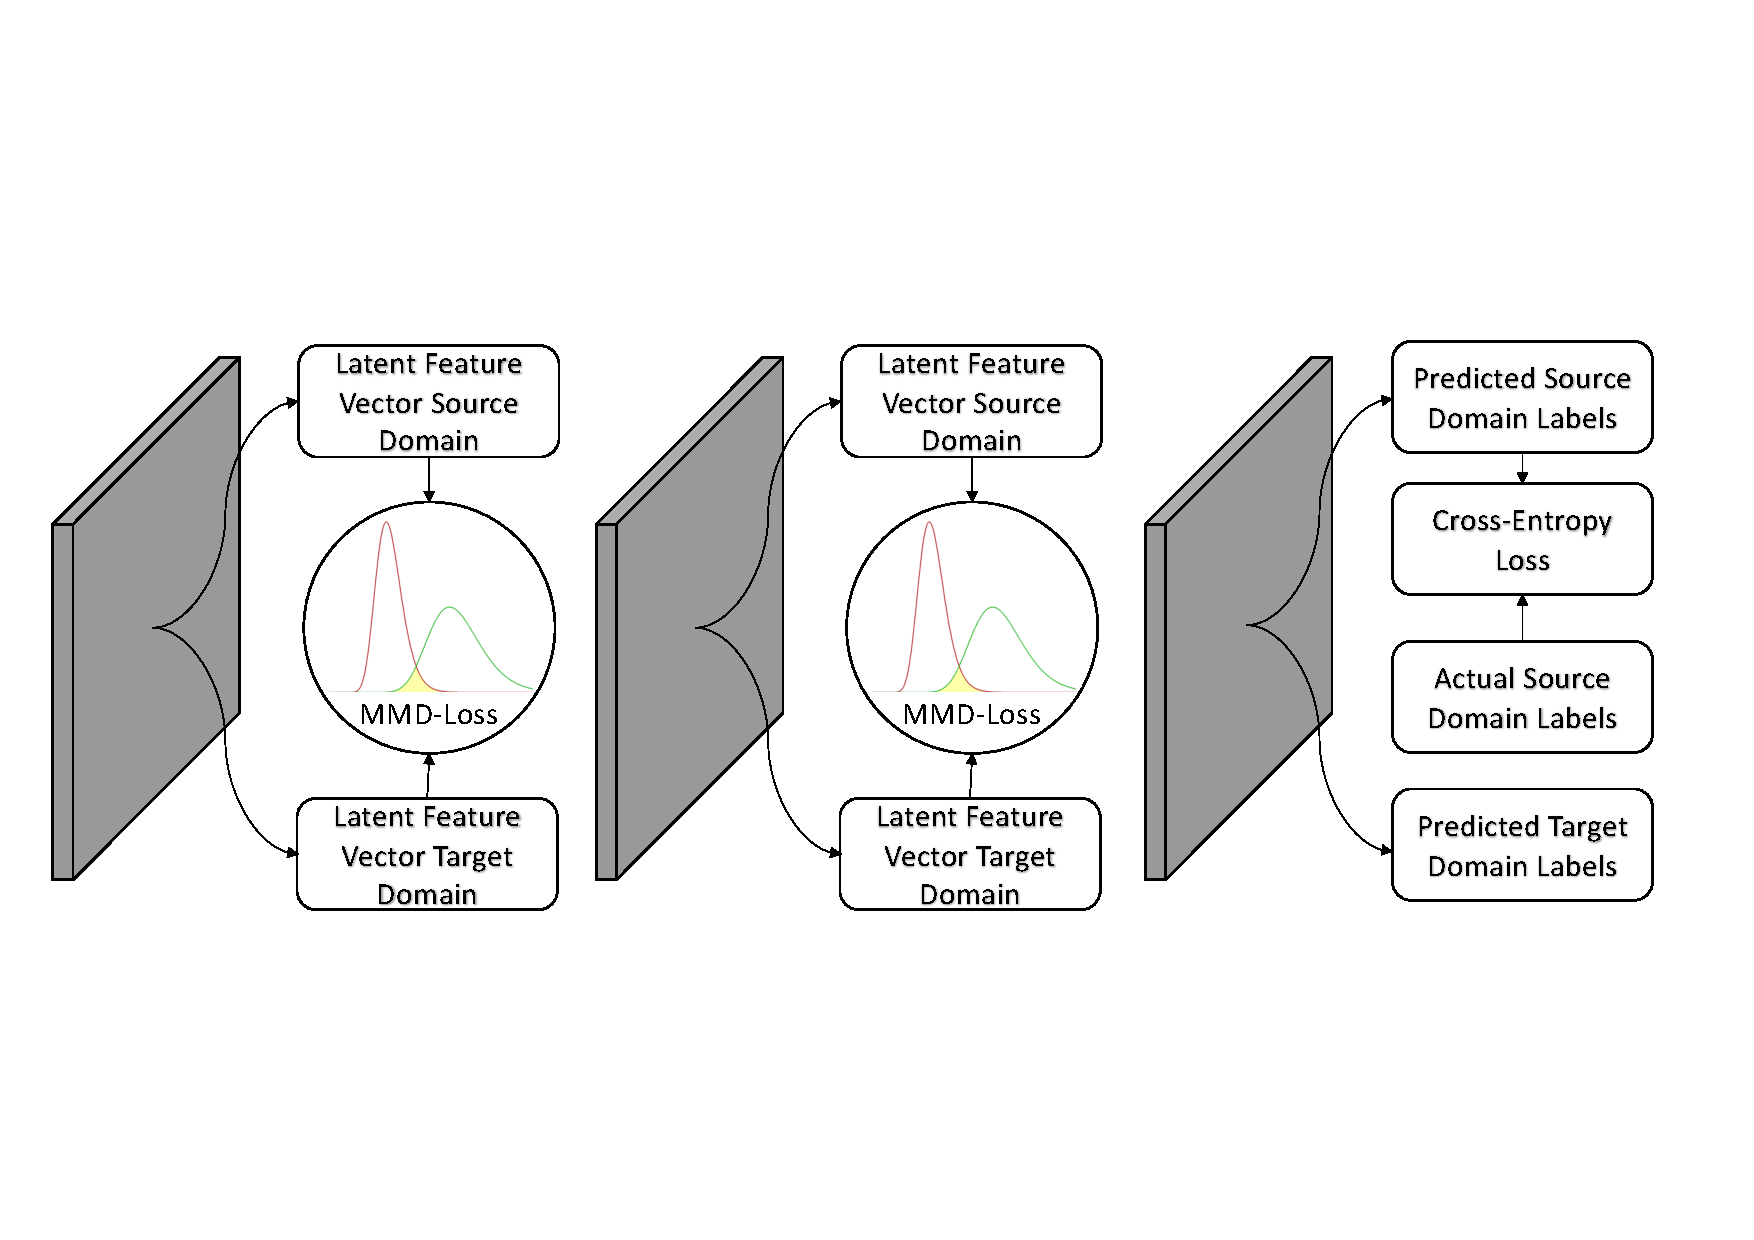
\includegraphics[width=1\textwidth]{MMD_loss_visualization.pdf}
  \caption {Cross Entropy Loss and MMD Loss in Neural Networks} \label{fig:MMD_Loss_and_CE_loss}
\end{figure}
 
A total loss must be specified by defining a weighted average between MMD and source cross entropy loss. The weighting factor GAMMA is a hyperparameter, which need to be defined beforehand. The total loss is defined as following:

\begin{align}
    \mbox{Total Loss} = \mbox{Source Cross-Entropy Loss} + \mbox{GAMMA} * \mbox{MMD Loss}
\end{align}.

The model training is separated in two phases. In a first phase the Total Loss is applied on the whole network. An ADAM optimizer is used with different learning rates for the layers Conv1 - FC1 and FC2 - FC3. In a second phase just the CE loss is applied to optimize the final two fully connected layers. Two-thirds of the train data is used in the first and one-third for the second train phase. The application of two different optimizers is visualized in fig. \ref{fig:proposed_model}. In general the training is repeated until the maximum number of epochs is reached. After the training is completed the model can be used to predict the health condition state of unseen source and target domain samples. 

\begin{figure}[H]
  \centering
  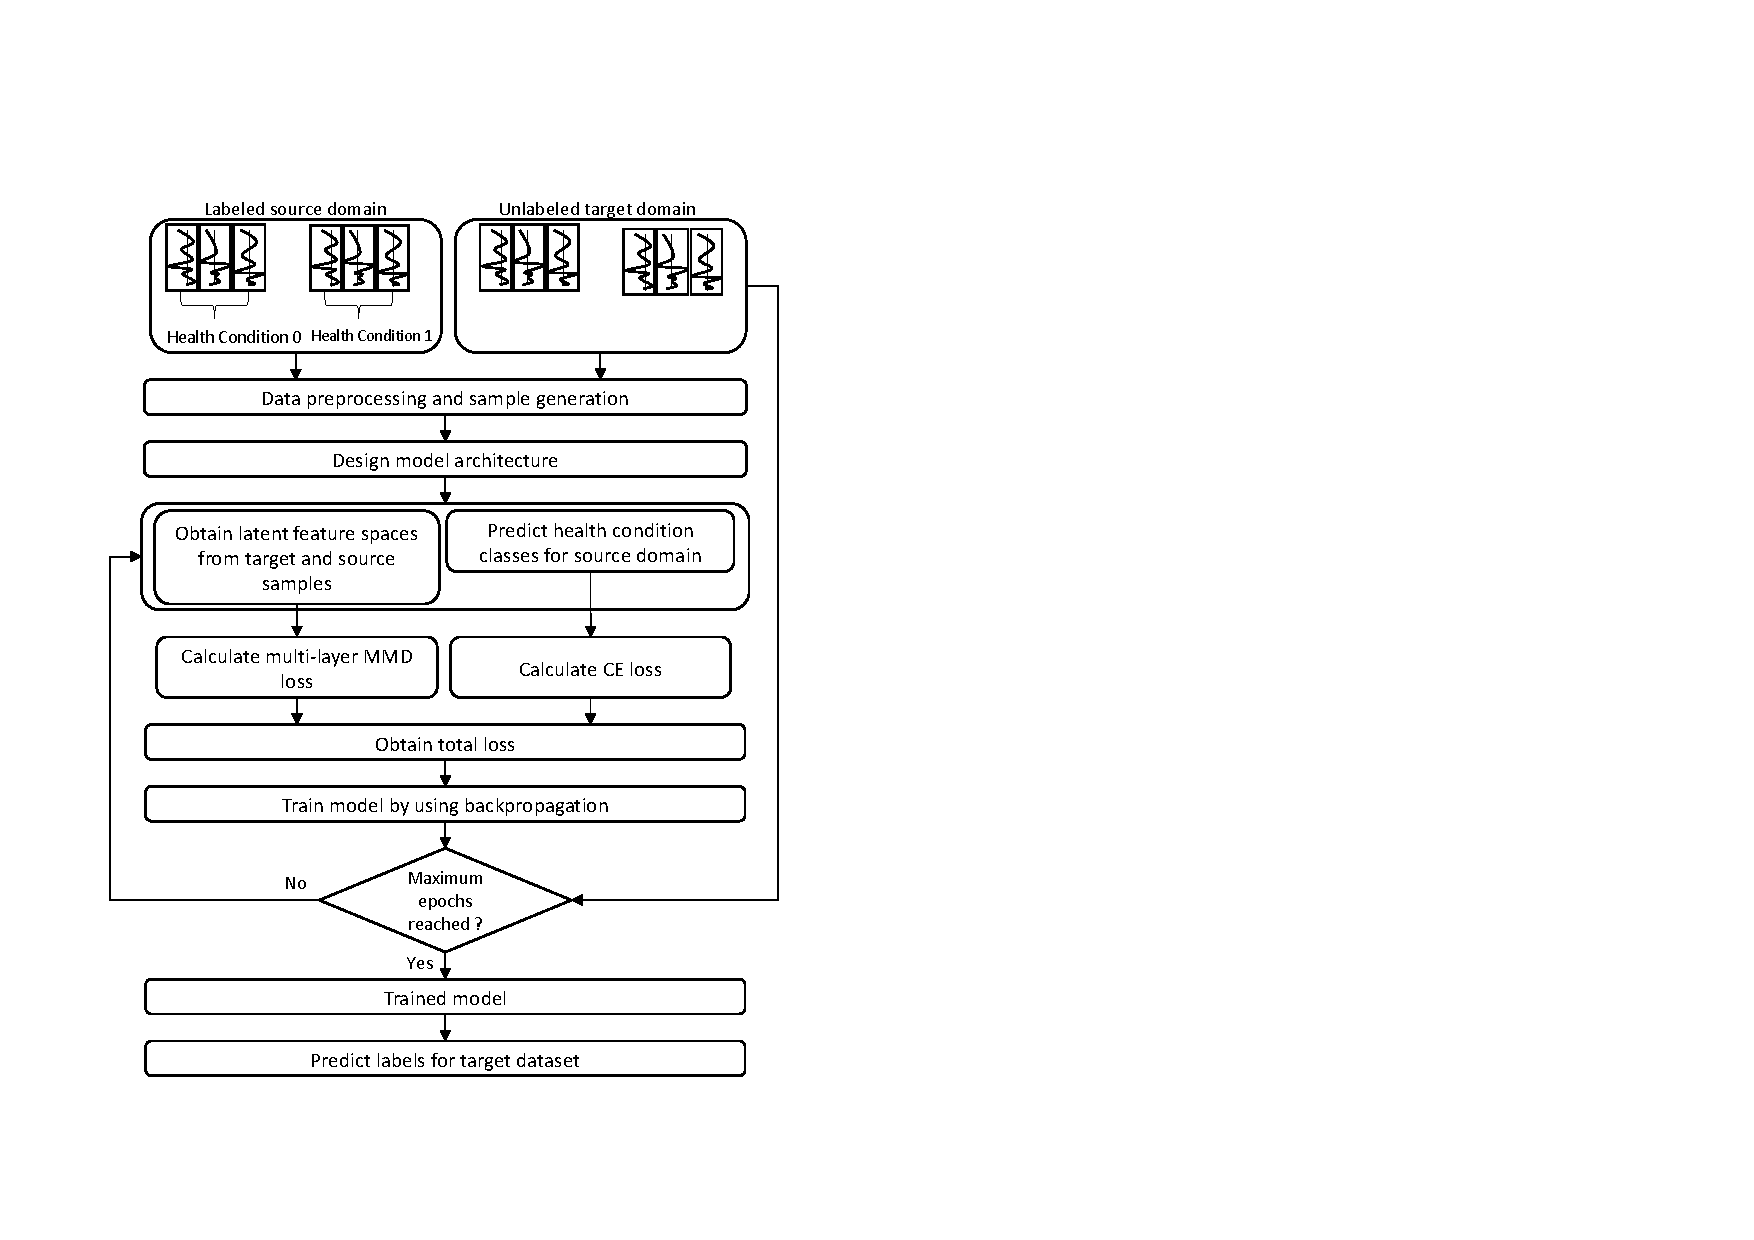
\includegraphics[width=0.8\textwidth]{training_process_mmd.pdf}
  \caption {Model training iteration} \label{fig:Training_Process_MMD}
\end{figure}

